\documentclass[t]{beamer}
\usetheme{Copenhagen}
\setbeamertemplate{headline}{} % remove toc from headers
\beamertemplatenavigationsymbolsempty

\usepackage{amsmath, array, tikz, bm, pgfplots, tcolorbox, graphicx, venndiagram, color, colortbl, xfrac}
\pgfplotsset{compat = 1.16}
\usepgfplotslibrary{statistics}
\usetikzlibrary{calc}

\title{Hypothesis Testing}
\subtitle{Single Sample Mean}
\author{}
\date{}

\AtBeginSection[]
{
  \begin{frame}
    \frametitle{Objectives}
    \tableofcontents[currentsection]
  \end{frame}
}

\begin{document}

\pgfmathdeclarefunction{gauss}{2}{%
  \pgfmathparse{1/(#2*sqrt(2*pi))*exp(-((x-#1)^2)/(2*#2^2))}%
}

\begin{frame} 
\maketitle
\end{frame}

\begin{frame}
Student's $t$ distribution
Degrees of Freedom: $n-1$ --> As deg. of freedom grow, t distribution becomes more normal.
$t = \frac{\overline{x}-\mu}{\sigma/\sqrt{n}}$

\end{frame}

\begin{frame}{Student's $t$ Test}
While the $z$ test for a population mean may be a good introduction to hypothesis testing, it doesn't hold much use in the real world. \newline\\	\pause

After all, how likely is it that you know for certain what the population standard deviation, $\sigma$, is, but you still have doubts about the population mean?	\newline\\	\pause

William Sealy Gosset, under the pseudonym \textit{Student}, created a hypothesis test for the population mean when the population standard deviation is unknown.
\end{frame}

\begin{frame}{Assumptions for Using the $t$ Test for a Population Mean}
\textbf{Assumptions:} 
\begin{itemize}
	\item<2-> The sample come from a normally distributed population; especially important for small sample sizes
	\item<3-> Sample was obtained randomly
\end{itemize}
\end{frame}

\begin{frame}{Degrees of Freedom}
The \textbf{degrees of freedom} of a sample size $n$ is given as $n - 1$.	\pause

\begin{center}
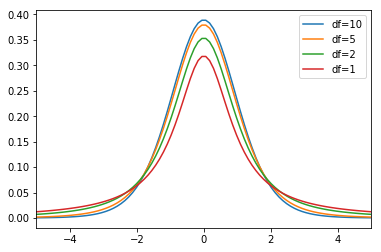
\includegraphics[scale=0.6]{../Images/t_distribution_df.png}
\end{center}
\pause

As the degrees of freedom grow, the $t$ distribution becomes more normal.
\end{frame}

\begin{frame}{Summary Stats}
Similar to a $z$ score, the test statistic $t$ can be found by calculating
\[t = \frac{\overline{x}-\mu}{s/\sqrt{n}}\]
\pause
$p$-value can be calculated using the test statistic and area under the curve. \newline\\	\pause
Confidence intervals for $t$ distribution are given by
\[\overline{x} \pm t_{\alpha/2}\left(\frac{s}{\sqrt{n}}\right)\]
where the degrees of freedom help determine the value of $t_{\alpha/2}$
\end{frame}

\begin{frame}{Am I Going to Be OK With This?}
If you understood the concepts and ideas behind the hypothesis testing we've done (in particular, being able to work with test statistics and critical values, $p$-values, or confidence intervals) then you should be alright with this section.	\newline\\	\pause

Quite frankly, just about all of the remaining material regarding hypothesis testing is just a variation on that theme.		\newline\\	\pause

Remember, most modern statistics uses computers or other technology to crunch the numbers. \newline\\	\pause

In the grand scheme of things, it's more valuable to be able to \emph{interpret those results}.
\end{frame}

\begin{frame}{Example 1}
% Given summary stats n >= 30

\end{frame}

\begin{frame}{Example 2}
% Raw Data n < 30
\end{frame}

\end{document}